\chapter{Metodología}\label{cap3}

\section{Liberías de Python}

Python \cite{python} es un lenguaje de programación interpretado de alto nivel que cuenta con multitud de librerías útiles para el análisis y la ciencia de datos. En este proyecto, las librerías utilizadas son:

\begin{itemize}
	\item Pandas.
	\item Scikit-learn.
	\item Matplotlib.
	\item Darts.
\end{itemize}

Pandas \cite{pandas} es una libería que permite el uso de \textit{dataframes}, unas estructuras de datos tabulares basada en columnas e índices, que permiten realizar multitud de operaciones. Scikit-learn \cite{scikit-learn} es una librería de aprendizaje automático muy completa, de la cual en este trabajo se utiliza sus herramientas para el cálculo de métricas de errores y el escalador de datos \textit{MinMaxScaler}. Matplotlib \cite{matplotlib} por su parte es la libería base para la creación de gráficas en Python.

Darts \cite{darts} merece una mención especial, ya que es la base del proyecto. Se trata de una librería \textit{open-source} creada por la empresa suiza Unit8. Está especializada en la realización de predicciones en series temporales o \textit{forecasting}. Cuenta con multitud de modelos integrados, desde probabilísticos como ARIMA hasta modelos de \textit{deep learning} basados en PyTorch \cite{pytorch}. Simplifica el uso de distintos modelos utilizando un esquema común para entrenamiento y predicción, permitiendo realizar experimentos con múltiples modelos con facilidad. Cuenta además con herramientas tanto para el preprocesamiento de los datos como para el análisis posterior.

\section{Series de datos de estudio}

En la empresa de recambios de automóvil de estudio, las distintas referencias se agrupan en familias de productos para recibir un tratamiento común independientemente de la marca. Por ejemplo, todas las referencias únicas referidas a baterías pertenecen a la familia de baterías. Los datos que se obtienen del ERP son el agrupado de ventas diarias de cada familia de estudio. Las familias de producto utilizadas en este estudio son las siguientes:

\begin{itemize}
    \item Baterías.
    \item Filtros.
    \item Aceites.
    \item Limpiaparabrisas.
\end{itemize} 

En cuanto al rango de fechas de los datos se incluye desde el inicio de la empresa a mediados de 2008 hasta la mitad del año 2024. Para evitar el efecto del comienzo de la empresa y tomar los años completos, los datos se toman desde el 1 de enero de 2012 hasta el 31 de diciembre de 2023, dejando la primera mitad del año 2024 como test para los modelos. Además, como los días de apertura son de lunes a viernes, se excluyen los fines de semana para facilitar el trabajo a los modelos. Sin embargo, para mantener coherencia entre todos los datos, se incluyen los días festivos que sea entre semana, que tendrán 0 unidades vendidas.

Los datos se encuentran en un archivo .csv y se cargan en Python en un \textit{DataFrame} de la librería Pandas \cite{pandas}. En el Código \ref*{ej-codcarga} se muestra un ejemplo de la carga de los datos de la familia de filtros. 

\lstinputlisting[caption=Carga de datos, label={ej-codcarga}]{codigos/carga_datos.py}

A continuación, en la Tabla \ref*{3-cabezafiltros} se observa una muestra con los cinco primeros datos como referencia de la estructura de los datos de las series.

\begin{table}[H]
	\ttabbox[\FBwidth]
	{\caption{Cabeza de la serie histórica de ventas de filtros}\label{3-cabezafiltros}}
	{\begin{tabular}{|c|c|}
		\hline
        \textbf{Fecha} & \textbf{Unidades vendidas} \\
        \hline
        2010-01-01 & 0 \\
        \hline
        2010-01-04 & 4 \\
        \hline
        2010-01-05 & 3 \\
        \hline
        2010-01-06 & 0 \\
        \hline
        2010-01-07 & 10 \\
        \hline
	\end{tabular}}
\end{table}


\subsection{Baterías}

Las baterías forman un grupo de producto el cual resulta relevante de estudio, ya que son un elemento común a todos los vehículos que se puede considerar consumible, ya que con el tiempo se degradan y es necesaria su sustitución. Además, son un elemento perecedero y por ello es necesario que pasen en el almacén el menor tiempo posible para evitar posibles fallos y, posteriores devoluciones por garatía. También hay que tener en cuenta que las baterías son productos más voluminosos y pesados, por lo que el coste de inventario es superior a la media de los demás productos.

En la Figura \ref*{3-graf_baterias}, se observa una gráfica de la serie temporal, donde se muestra una clara tendencia al alza y cierta estacionalidad. Además, a destacar el bajón de ventas producidas por el confinamiento durante el COVID y el posterior incremento de las ventas al ser diferidas.

\begin{figure}[H]
	\ffigbox[\FBwidth] {
	\caption{Gráfica de la serie temporal de ventas de baterías}\label{3-graf_baterias}
	}
	{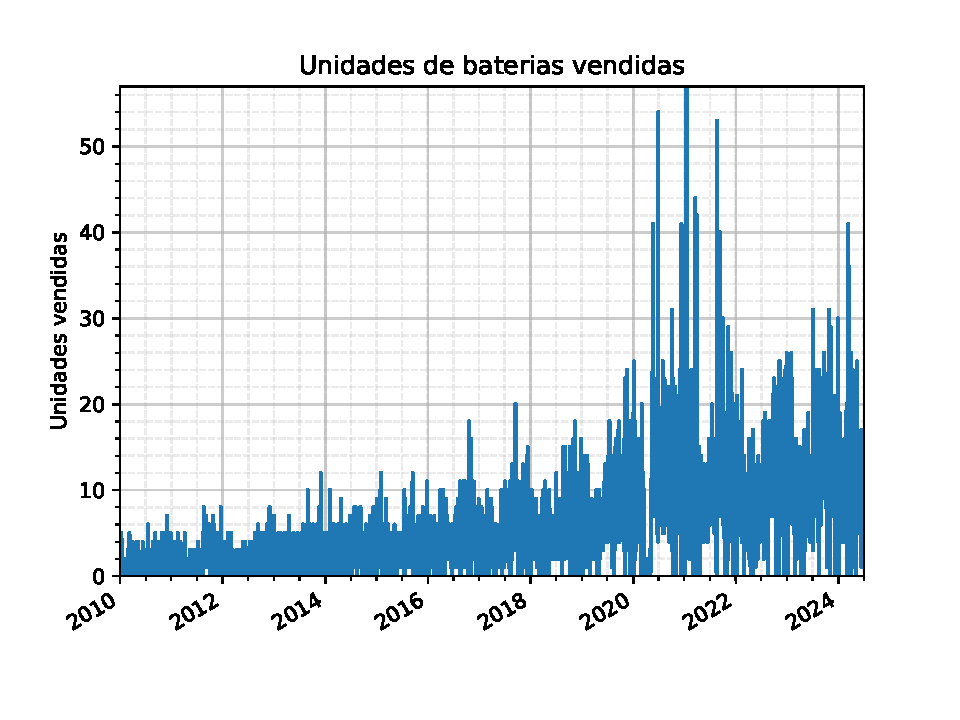
\includegraphics[width=0.75\textwidth]{imagenes/grafica_baterias.pdf}}
\end{figure}

Utilizando la librería Prophet \cite{prophet}, se desglosa la estacionalidad de la serie temporal, mostrada en la Figura \ref*{3-comp_baterias}. La primera subgráfica muestra la tendencia al alza en las ventas de esta familia. La segunda, muestra la estacionalidad intrasemanal, donde muestra que la mayoría de ventas se producen a comienzo de semana. En la última, la estacionalidad anual muestra que las ventas entorno al mes de abril son las más bajas del año, mientras que a partir de septiembre se incrementan considerablemente.

\begin{figure}[H]
	\ffigbox[\FBwidth] {
	\caption{Gráfica de componentes de la serie de baterías}\label{3-comp_baterias}
	}
	{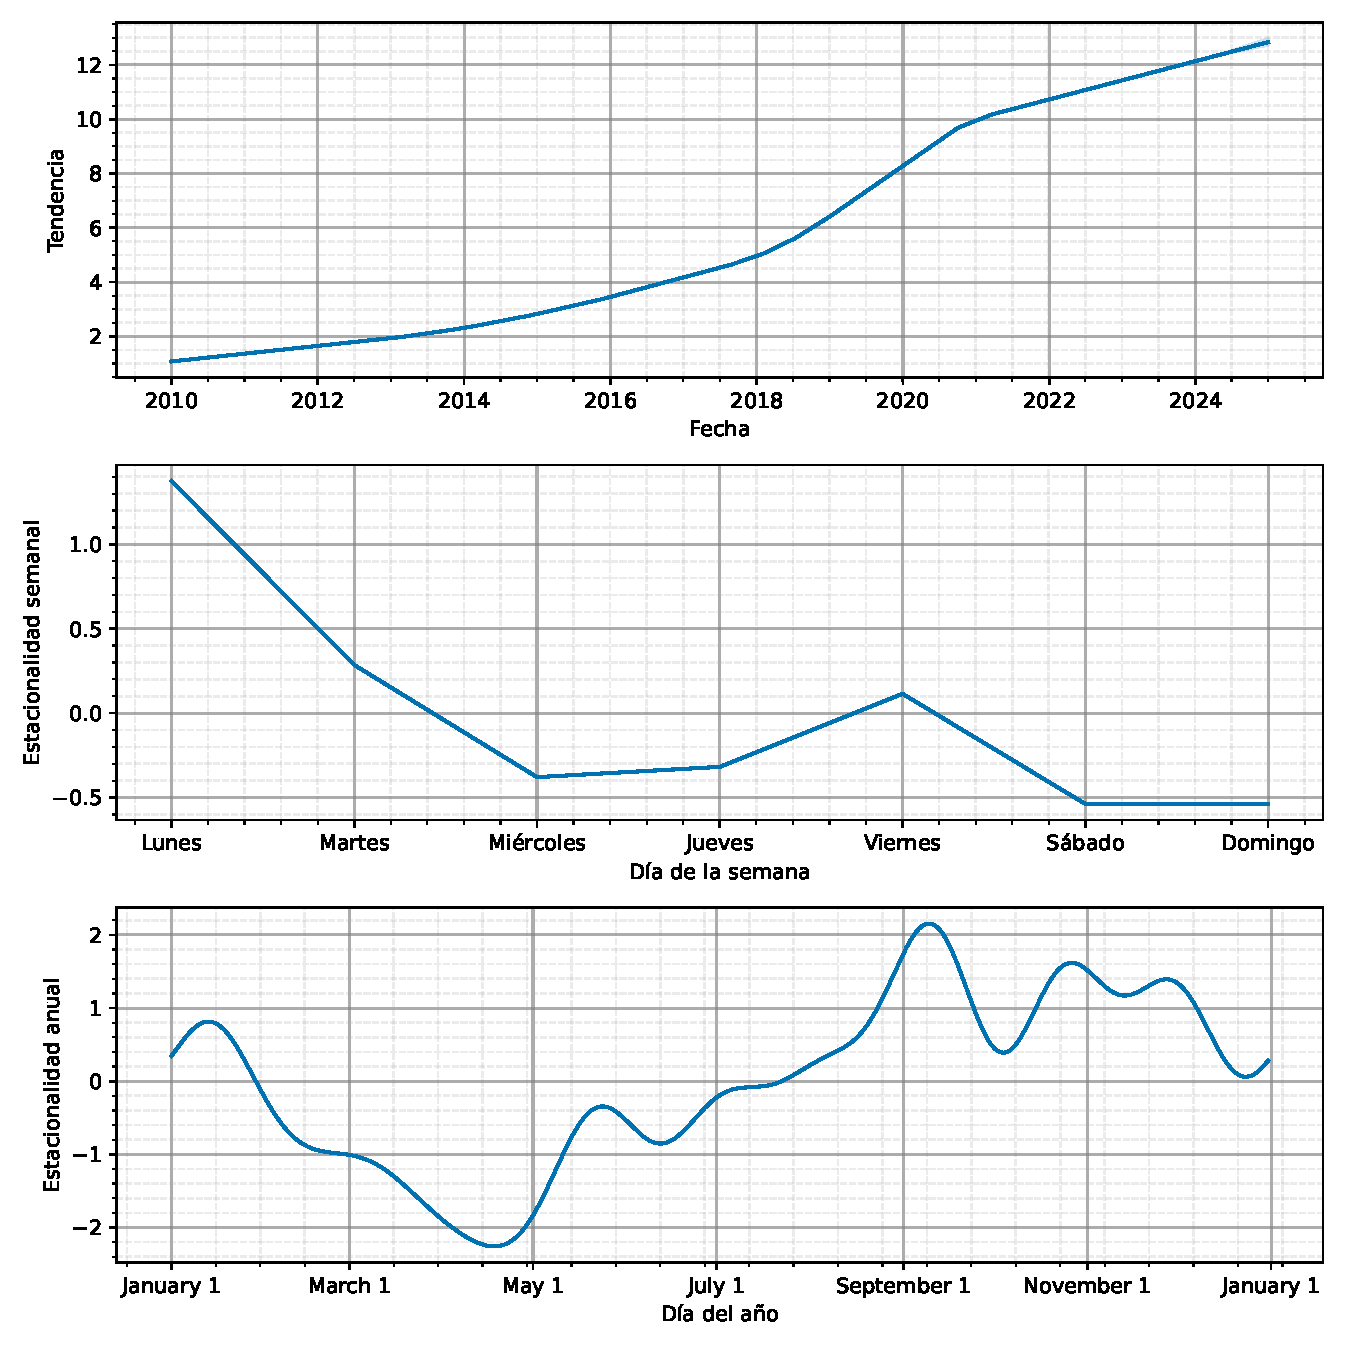
\includegraphics[width=0.75\textwidth]{imagenes/comps_baterias.pdf}}
\end{figure}


\subsection{Filtros}

Los filtros son el consumible por excelencia de los vehículos con motores de combustión, ya que la sustitución periódica de filtros como el de aceite y el de combustible es esencial para alargar la vida útil del motor. Además, también hay filtros como el de aire que se encuentran también en vehículos eléctricos. Por esto, se conforma una familia de producto que tiene un alto volumen de ventas.

En la Figura \ref*{3-graf_filtros} se observa el histórico de datos de la familia de producto. No se aprecia tanta estacionalidad como en el caso de las baterías, pero la tendencia al alza es bastante clara en los primeros años, con un estancamiento a partir del año 2020.

\begin{figure}[H]
	\ffigbox[\FBwidth] {
	\caption{Gráfica de la serie temporal de ventas de filtros}\label{3-graf_filtros}
	}
	{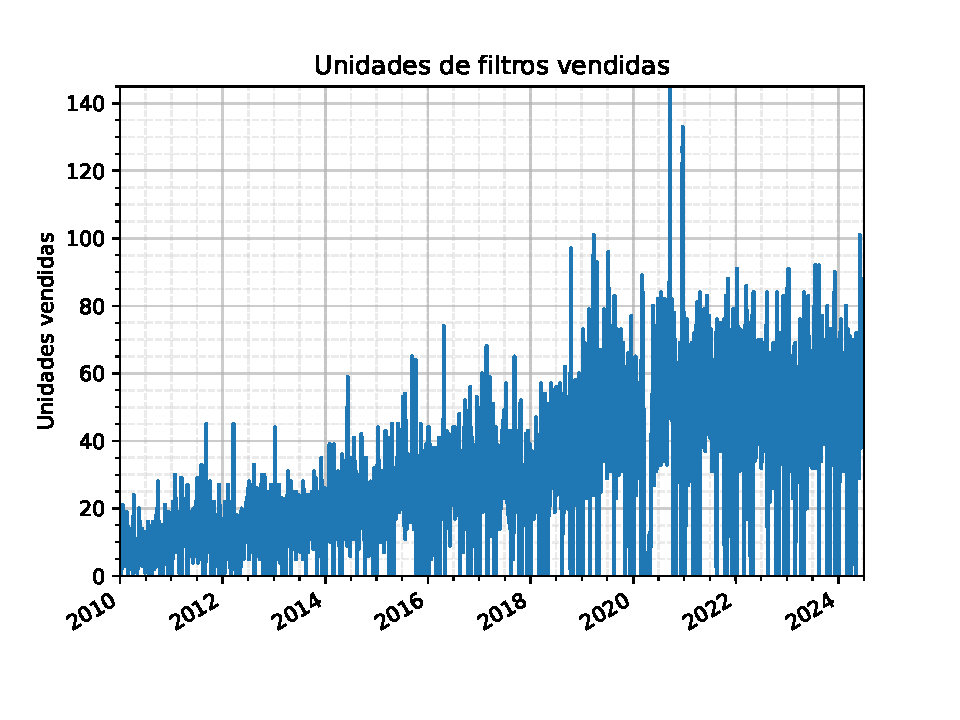
\includegraphics[width=0.75\textwidth]{imagenes/grafica_filtros.pdf}}
\end{figure}

Desglosando los componentes estacionales, no se observa una estacionalidad muy marcada a nivel semanal, pero sí a nivel anual, donde la mayoría de mantenimientos se realizan previos a períodos vacacionales.

\begin{figure}[H]
	\ffigbox[\FBwidth] {
	\caption{Gráfica de componentes de la serie de filtros}\label{3-comp_filtros}
	}
	{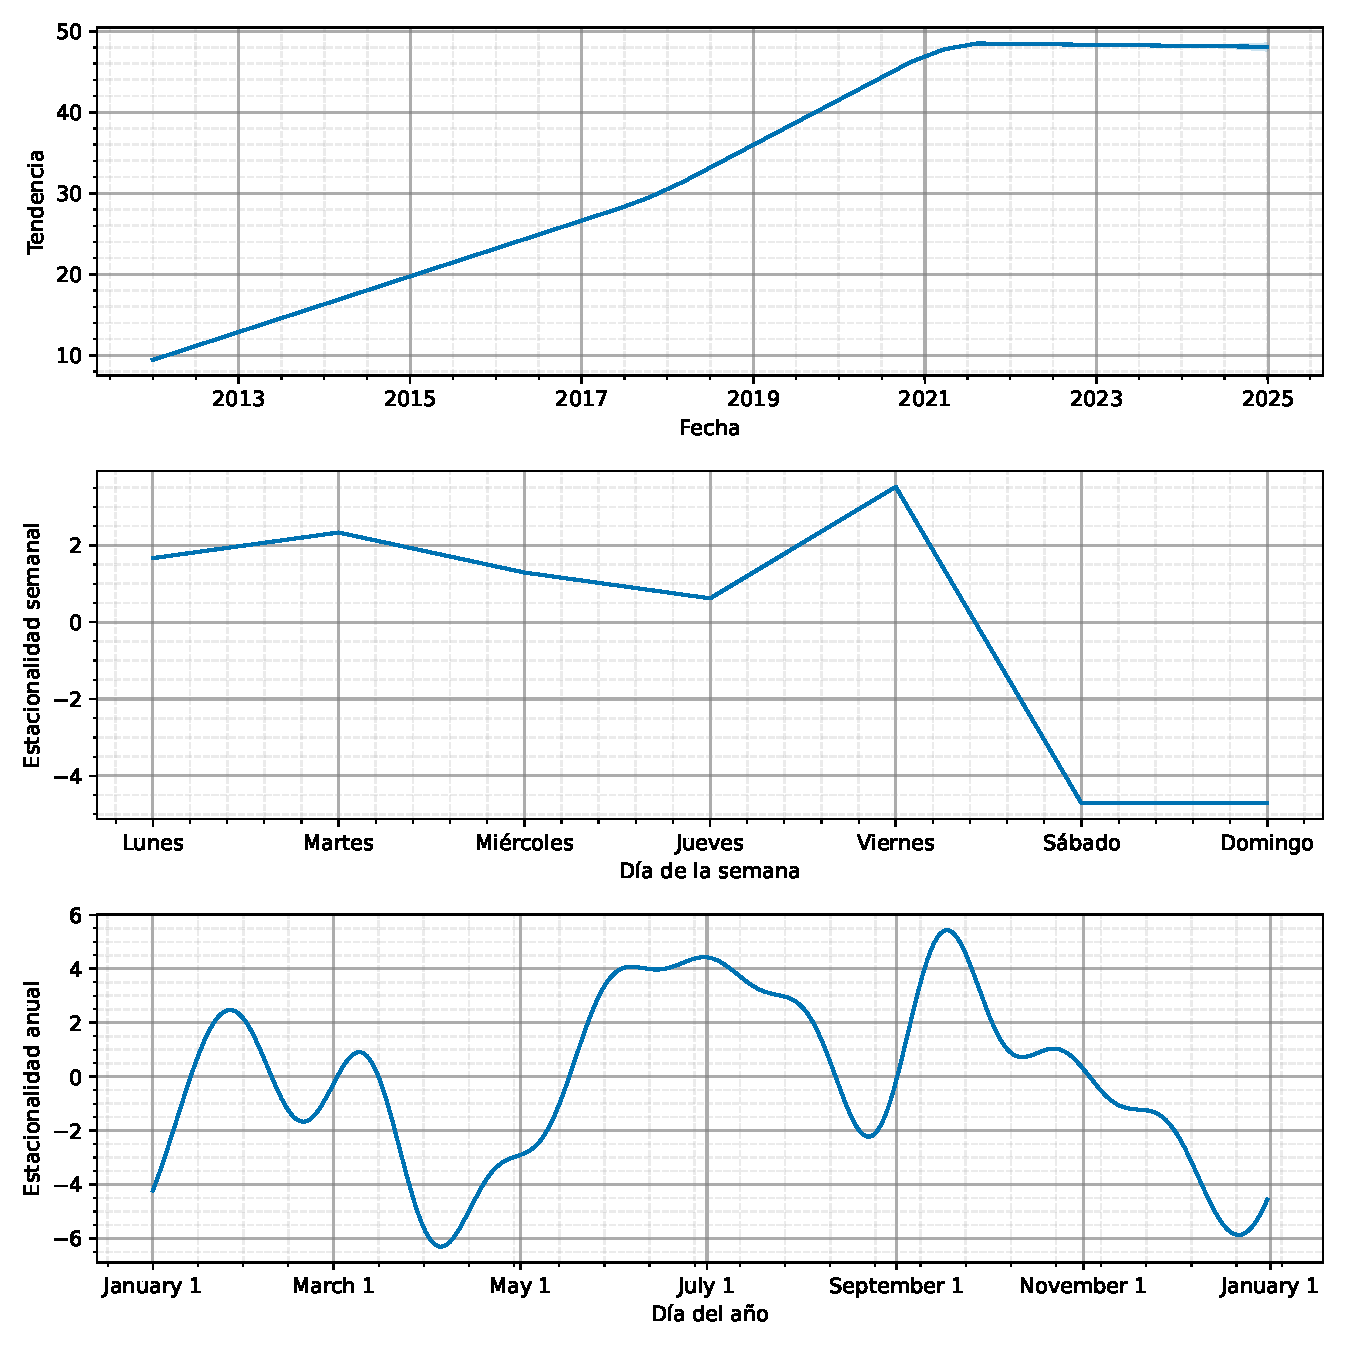
\includegraphics[width=0.75\textwidth]{imagenes/comps_filtros.pdf}}
\end{figure}

\subsection{Aceites}

Otra familia importante es la de los aceites industriales. Se trata de productos que suelen ser voluminosos y, al igual que los filtros, su sustitución es imprescindible para un correcto mantenimiento de vehículos térmicos y alargar su vida útil. En la Figura \ref*{3-graf_aceites} se muestra la gráfica de la serie histórica.

\begin{figure}[H]
	\ffigbox[\FBwidth] {
	\caption{Gráfica de la serie temporal de ventas de aceites}\label{3-graf_aceites}
	}
	{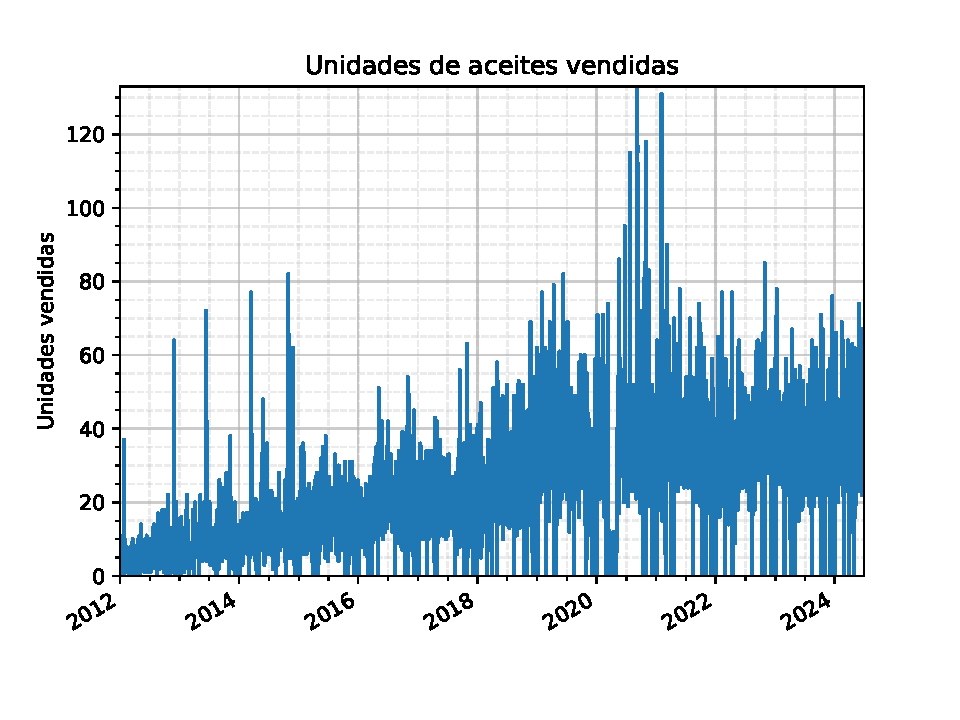
\includegraphics[width=0.75\textwidth]{imagenes/grafica_aceites.pdf}}
\end{figure}



\begin{figure}[H]
	\ffigbox[\FBwidth] {
	\caption{Gráfica de componentes de la serie de aceites}\label{3-comp_aceites}
	}
	{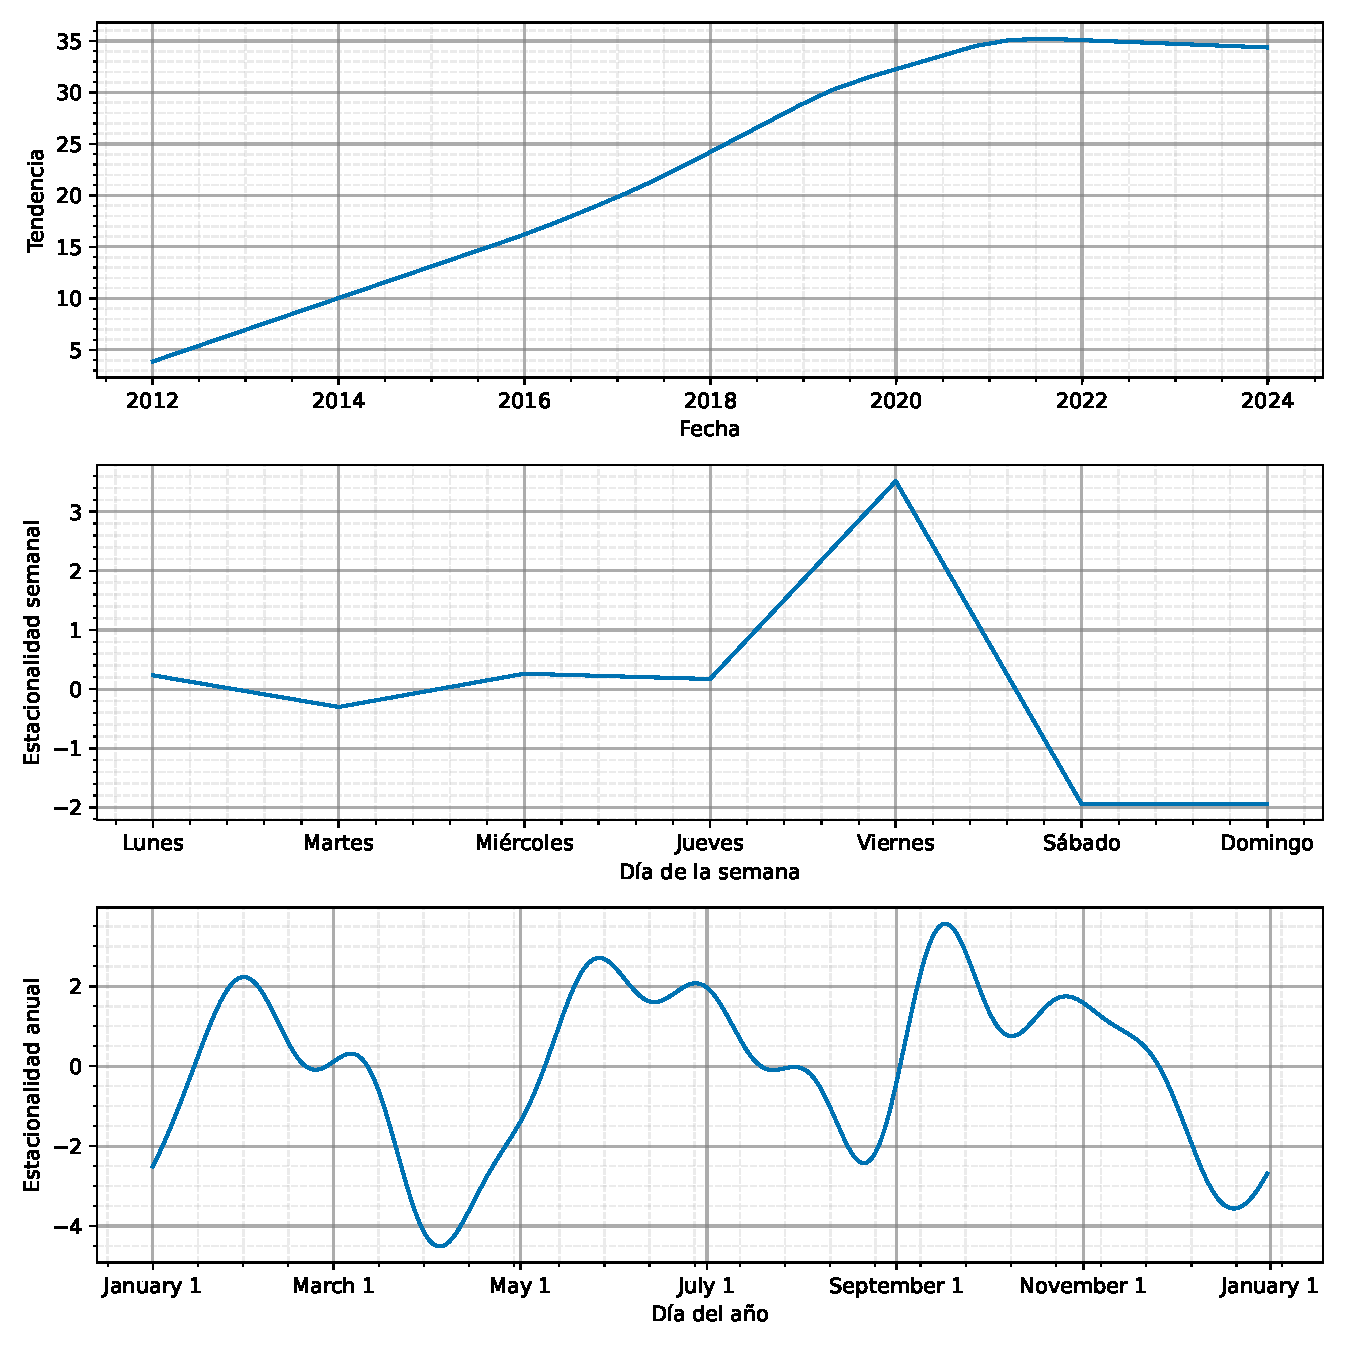
\includegraphics[width=0.75\textwidth]{imagenes/comps_aceites.pdf}}
\end{figure}

\subsection{Limpiaparabrisas}

Los limpiaparabrisas son un tipo de producto con una clara estacionalidad, ya que durante la época con mayor irradiación solar se deterioran en coches estacionados en la calle y se sustituyen cuando empieza la época de lluvias. En la Figura \ref*{3-graf_limpiaparabrisas}, se observa como hay picos intensos de demanda y valles marcados.

\begin{figure}[H]
	\ffigbox[\FBwidth] {
	\caption{Gráfica de la serie temporal de ventas de limpiaparabrisas}\label{3-graf_limpiaparabrisas}
	}
	{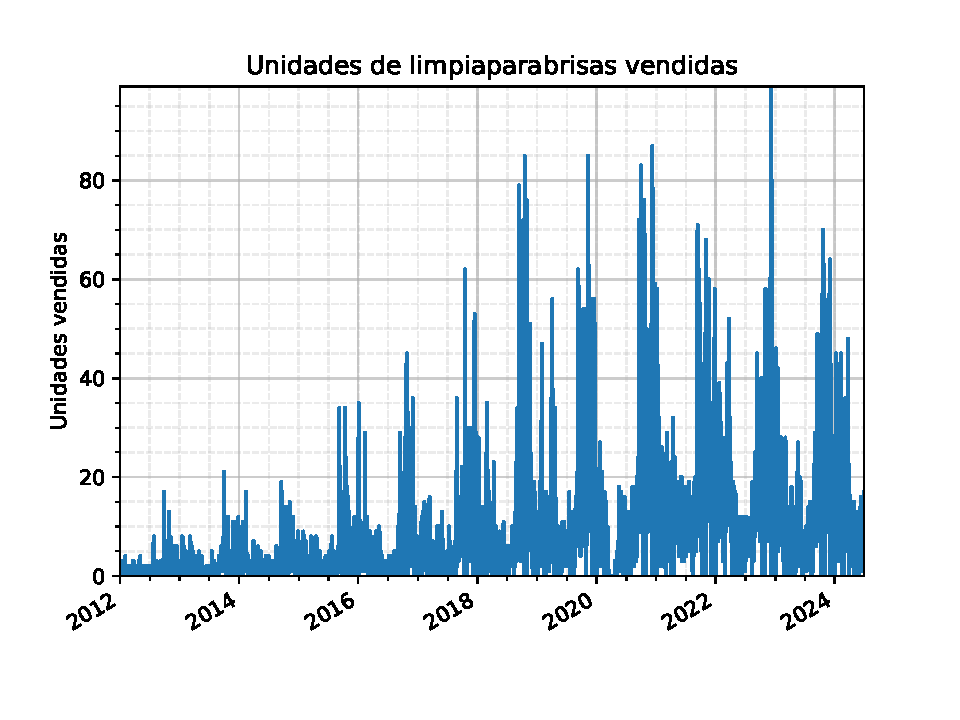
\includegraphics[width=0.75\textwidth]{imagenes/grafica_limpiaparabrisas.pdf}}
\end{figure}

En la Figura \ref*{3-comp_limpiaparabrisas} se observan el incremento de las ventas a lo largo de la serie histórica y la estacionalidad que concenctra las ventas después de la época de verano.

\begin{figure}[H]
	\ffigbox[\FBwidth] {
	\caption{Gráfica de componentes de la serie de limpiaparabrisas}\label{3-comp_limpiaparabrisas}
	}
	{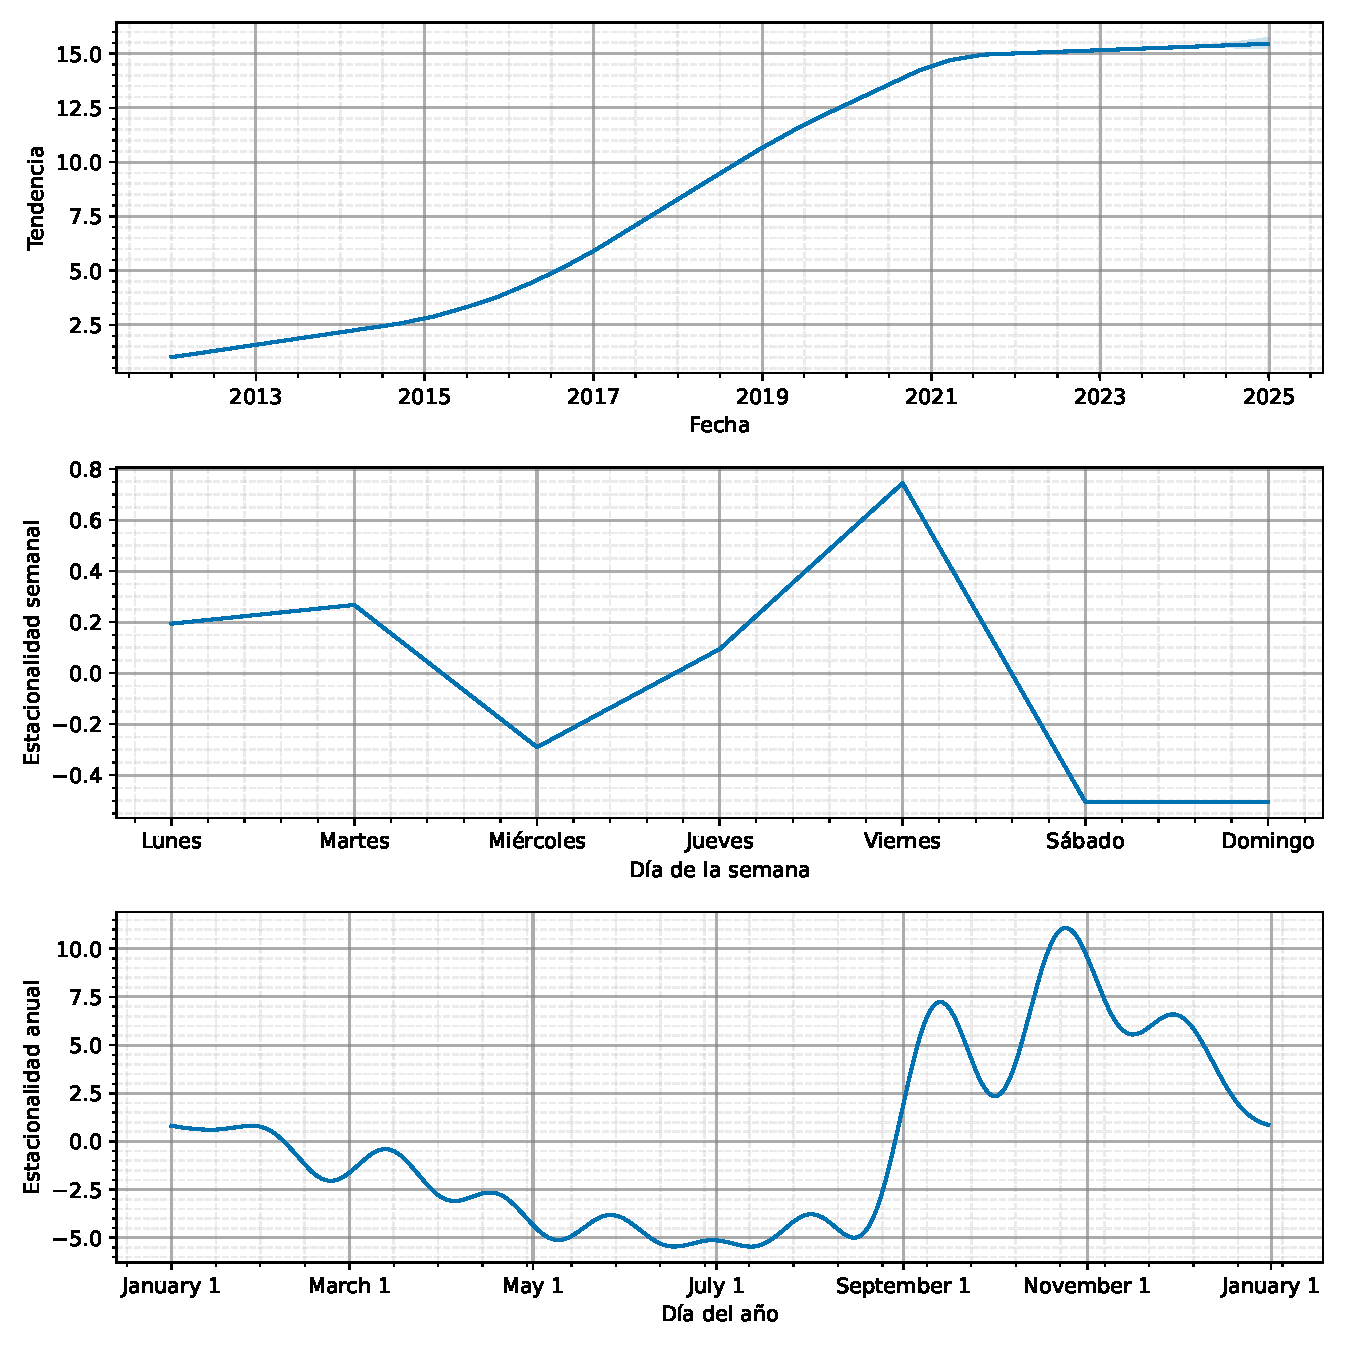
\includegraphics[width=0.75\textwidth]{imagenes/comps_limpiaparabrisas.pdf}}
\end{figure}


\section{Regresores externos}

A pesar de que el enfoque de las predicciones es univariable, ya que solo se busca predecir el valor de las ventas, es posible añadir regresores externos o \textit{covariates} para mejorar los resultados. Estos regresores pueden ser pasados, futuros o estáticos. En el caso de estudio presente, se utilizan regresores pasados.

\subsection{Días festivos}

Los días festivos las tiendas permanecen cerradas, por lo que las ventas son cero. Como las series de datos de estudio incluyen todos los días de lunes a viernes incluyendo los festivos, es buena idea añadir como regresor una serie donde se indique los días que son festivos. En este sentido, la librería Darts añade la funcionalidad de añadir una una serie extra con los días laborables de España y, además, de Andalucía. Se trata de una serie con una variable binaria donde 1 indica que es día festivo y 0 indica que no lo es. Se puede observar en la Figura \ref*{3-dias_festivos} los días festivos durante el rango de fechas del caso de estudio.

\begin{figure}[H]
	\ffigbox[\FBwidth] {
	\caption{Días festivos de España y Andalucía}\label{3-dias_festivos}
	}
	{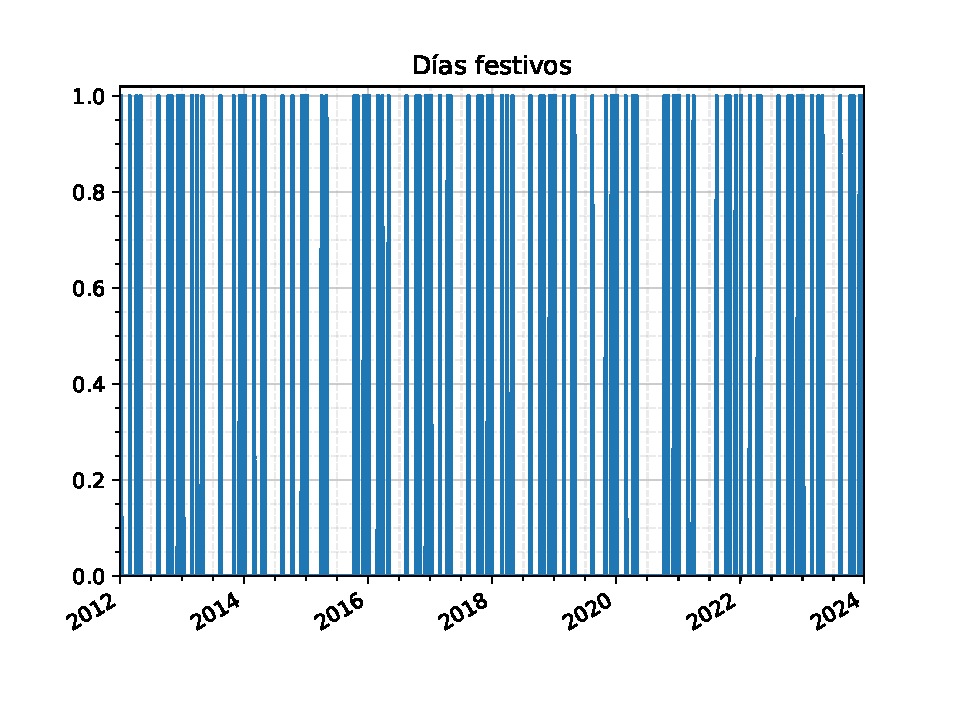
\includegraphics[width=0.75\textwidth]{imagenes/grafica_holidays.pdf}}
\end{figure}

\subsection{Meteorología}

\subsection{Precio del carburante}

El precio de la gasolina y del diésel influye en la industria de la automoción en gran medida, ya que su valor incrementa el coste de la movilidad en vehículos térmicos. Por ello, su precio puede influir en la industria del \textit{aftermarket} del automóvil al verse reducido el uso de los vehículos. Por ello, es interesante utilizarlo como regresor durante el entrenamiento de los modelos.

Para ello, se utilizan datos obtenidos del Boletín del Petróleo de la Comisión Europea \cite{petrol} que provee datos semanales del precio de diversos combustibles en todos los países de la Unión Europea. Como el diésel y la gasolina son los carburantes más empleados en la mayoría de vehículos serán los empleados en el estudio. Los datos obtenidos son semanales mientras que nuestros datos son diarios, por lo que el valor de cada semana se extenderá a todos los días de esa semana. La Figura \ref*{3-precio_combustible} muestra la evolución del precio de ambos combustibles a lo largo del período del estudio.

\begin{figure}[H]
	\ffigbox[\FBwidth] {
	\caption{Evolución del precio del combustible en España}\label{3-precio_combustible}
	}
	{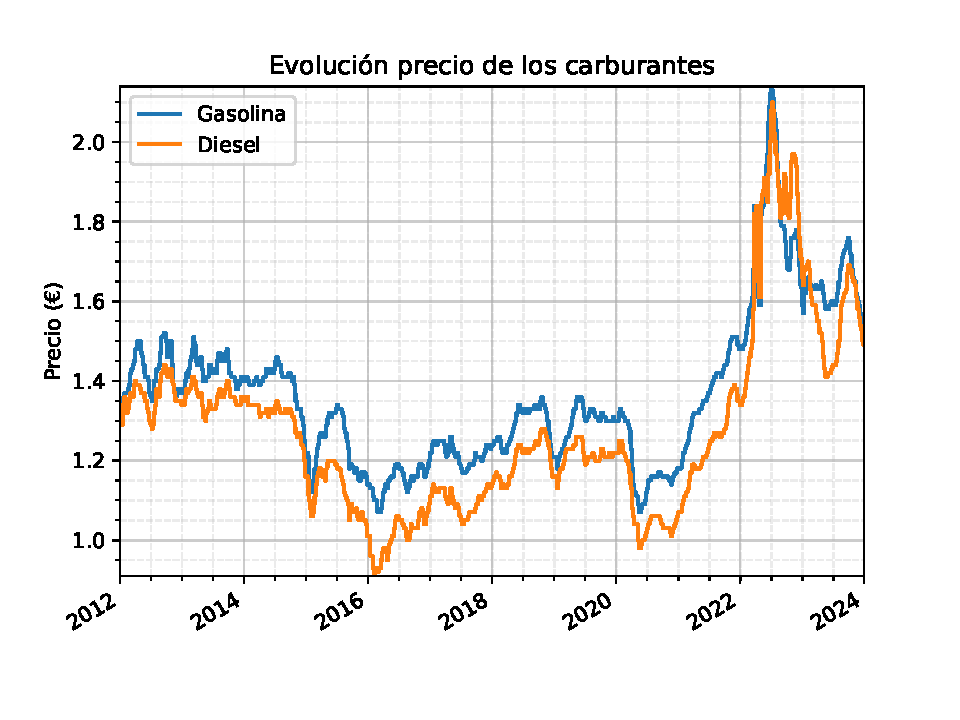
\includegraphics[width=0.75\textwidth]{imagenes/grafica_carburantes.pdf}}
\end{figure}

\section{Modelos}

\subsection{Prophet}

Prophet \cite{prophet} es una herramienta desarrollada por Facebook (ahora conocida como Meta) para el análisis de series temporales. Está especializada en datos que presentan patrones estacionales y tendencia. Está enfocada a ser fácil de usar y no requerir mucha configuración y se utiliza como librería en Python o R \cite{R}. El modelo incluido descompone la serie temporal en tendencia y estacionalidad. Además, permite añadir los festivos locales para mejorar las predicciones.

Se utiliza un modelo en el que la tendencia se modela de forma flexible, permitiendo cambios no lineales mediante \textit{changepoints}. Evita los valores atípicos y los datos faltantes, dando robustez al modelo frente a series temporales ruidosas o incompletas.

Su uso en este trabajo es de \textit{plug and play}, ya que se instancia la librería por defecto, a excepción de la especificación de los festivos de España (la librería no incluye la posiblidad de añadir los festivos de Andalucía).

Es necesario destacar que es el único modelo de los implementados que no depende de PyTorch \cite{pytorch}.

\subsection{RNN}
\subsection{N-BEATS y N-HiTS}
\subsection{TCN}
\subsection{DLinear y NLinear}
\subsection{TiDE}
\subsection{TSMixer}